\section{实验分析}
为了验证本文所提出的势能损失函数对于模型补全攻击的有效性,本文在多个数据集上进行了实验,并且与距离相关性损失~\cite{vepakomma2020nopeek,sunjiankai2022forward_embedding_protect}以及标签差分隐私(Label Differential Privacy)~\cite{wuruihan_2023_label_dp}的方法进行对比。
%
各个数据集和对应的模型介绍如下:
\begin{itemize}
    \item MNIST~\cite{mnist}:一个常用的手写数字数据集,是一个10分类的手写数字分类数据集,包含了60000个训练样本和10000个验证样本,每个样本为$28\times 28$的灰度图片。
    对应的模型是一个隐层大小为[128, 32]的全连接神经网络,激活函数采用LeakyReLU。
    
    \item Fashion-MNIST~\cite{fashion}:一个包含了10个类别的图片数据集,包含了7万张服饰相关的$28\times 28$大小的黑白图片。
    对应的模型是一个双层卷积加上双层全连接的模型,卷积层的通道数分别为[32, 64],卷积核大小分别为$[5, 3]$,每一个卷积层后面跟随LeakyReLU激活函数和大小为2的最大池化层。
    全连接层的维度为2304(卷积层提供的输入)-128-10(输出)。
    
    \item CIFAR-10~\cite{krizhevsky_2009_cifar}:一个包含了10个类别的6万张图片的彩色图片数据集,图片大小为$3\times 32\times 32$。
    对应的模型是ResNet-20模型~\cite{hekaiming2016resnet}。

    \item DBPedia~\cite{2007dbpedia}:一个文本分类数据集,在第\ref{chap:randomized_topk}章已经进行了介绍。
    我们采用TextCNN模型~\cite{kimyoon2014textcnn}进行分类,卷积核的大小为 $(3,4,5)$,并且使用Glove预训练词向量~\cite{pennington2014glove}。
    拆分层设置为最后的隐层,大小为300。
\end{itemize}
%

攻击者采用微调攻击和聚类攻击两种方法对训练完成的拆分学习模型进行攻击。
对于微调攻击,当拆分层为最后一层的时候,攻击者使用同类样本表征均值来初始化最后一层的权重。
对于聚类攻击,我们采用经典的$k$-平均($k$-Means)聚类算法~\cite{macqueen1967kmeans},并且给定类别个数。

所有实验都在装配有NVIDIA RTX 3090 GPU的服务器上进行,并使用不同的随机种子重复5次以上。
%
对于所有的任务,我们最多训练100轮模型,并在90-100轮中采用“早停(Early Stopping)”策略获取验证集最佳的模型,以保证原始损失函数和额外损失函数均被充分优化。
%
对于聚类攻击,我们采用Scikit-Learn库~\cite{pedregosa_2011_scikit}中的$k$-平均聚类算法,并采用默认参数。
%
我们将势能损失的权重从0.25变化到32,每次翻倍;
类似地,对于距离相关性损失,我们也把权重从1变化到32,每次翻倍;
对于标签差分隐私方法,我们将翻转的标签比例从0.01提高到0.16,每次翻倍。
%
我们默认将拆分层选为模型的最后一层,因为其最贴近模型的输出,但我们也汇报了拆分层选为其他层的实验结果。
%



\subsection{微调攻击}

我们测量了模型在测试集上的准确率,以及攻击者在泄漏的带标签数据上进行微调攻击得到的模型的准确率。
我们将拆分层为最后一层的结果和拆分层为中间其他层的结果分别汇报在\autoref{fig:peloss:fine-tuning}和\autoref{fig:peloss:fine-tuning-middle}中。
%
在拆分中间其他层的实验中,我们将MNIST任务的全连接神经网络的拆分层设置在第一个隐层处,将CIFAR-10任务的拆分层设置在第二个残差块(Residual Block)之后。

图中的数据点的深浅对应实验中势能损失函数/距离相关性损失函数的系数或标签翻转概率,颜色越深代表超参数的设定越偏向于保护隐私,越浅则代表超参数的设定越偏向于保留原始任务的准确率。
%
落在灰色区域的数据表示训练好的拆分学习模型实现了完美保护,也就是底部模型或隐层表征对于攻击者没有任何额外作用,攻击者对其实行攻击的效果未达到在泄漏的数据集上直接训练的效果。
%
如果数据点落在图的左下角,说明该实验降低了攻击准确率的同时保持了原始任务的准确率。

实验结果表明,如果不对拆分学习加以防护,则攻击者可以获得很高的攻击效果。
%
标签差分隐私、距离相关性损失和势能损失都能一定程度上降低攻击准确率,且势能损失的数据点大多落在对比方法的右下方,表明势能损失取得了更好的保护效果的同时又有更高的原始任务准确率。
%
同时,势能损失数据点连成的曲线较为平滑,可以很清楚展现出通过改变损失系数来权衡原始任务准确率和攻击效果的过程。与此同时,距离相关性损失的数据点则难以连成曲线,表明其效果难以控制。
%
此外,势能损失有最多的数据点落在完美保护区域,而其他方法落在完美保护区域的数据点则很少。
%
综上,对于微调攻击,在同等的原始任务准确率下,势能损失的防御效果显著高于其他方法。

\begin{figure}[h!]
    \centering
    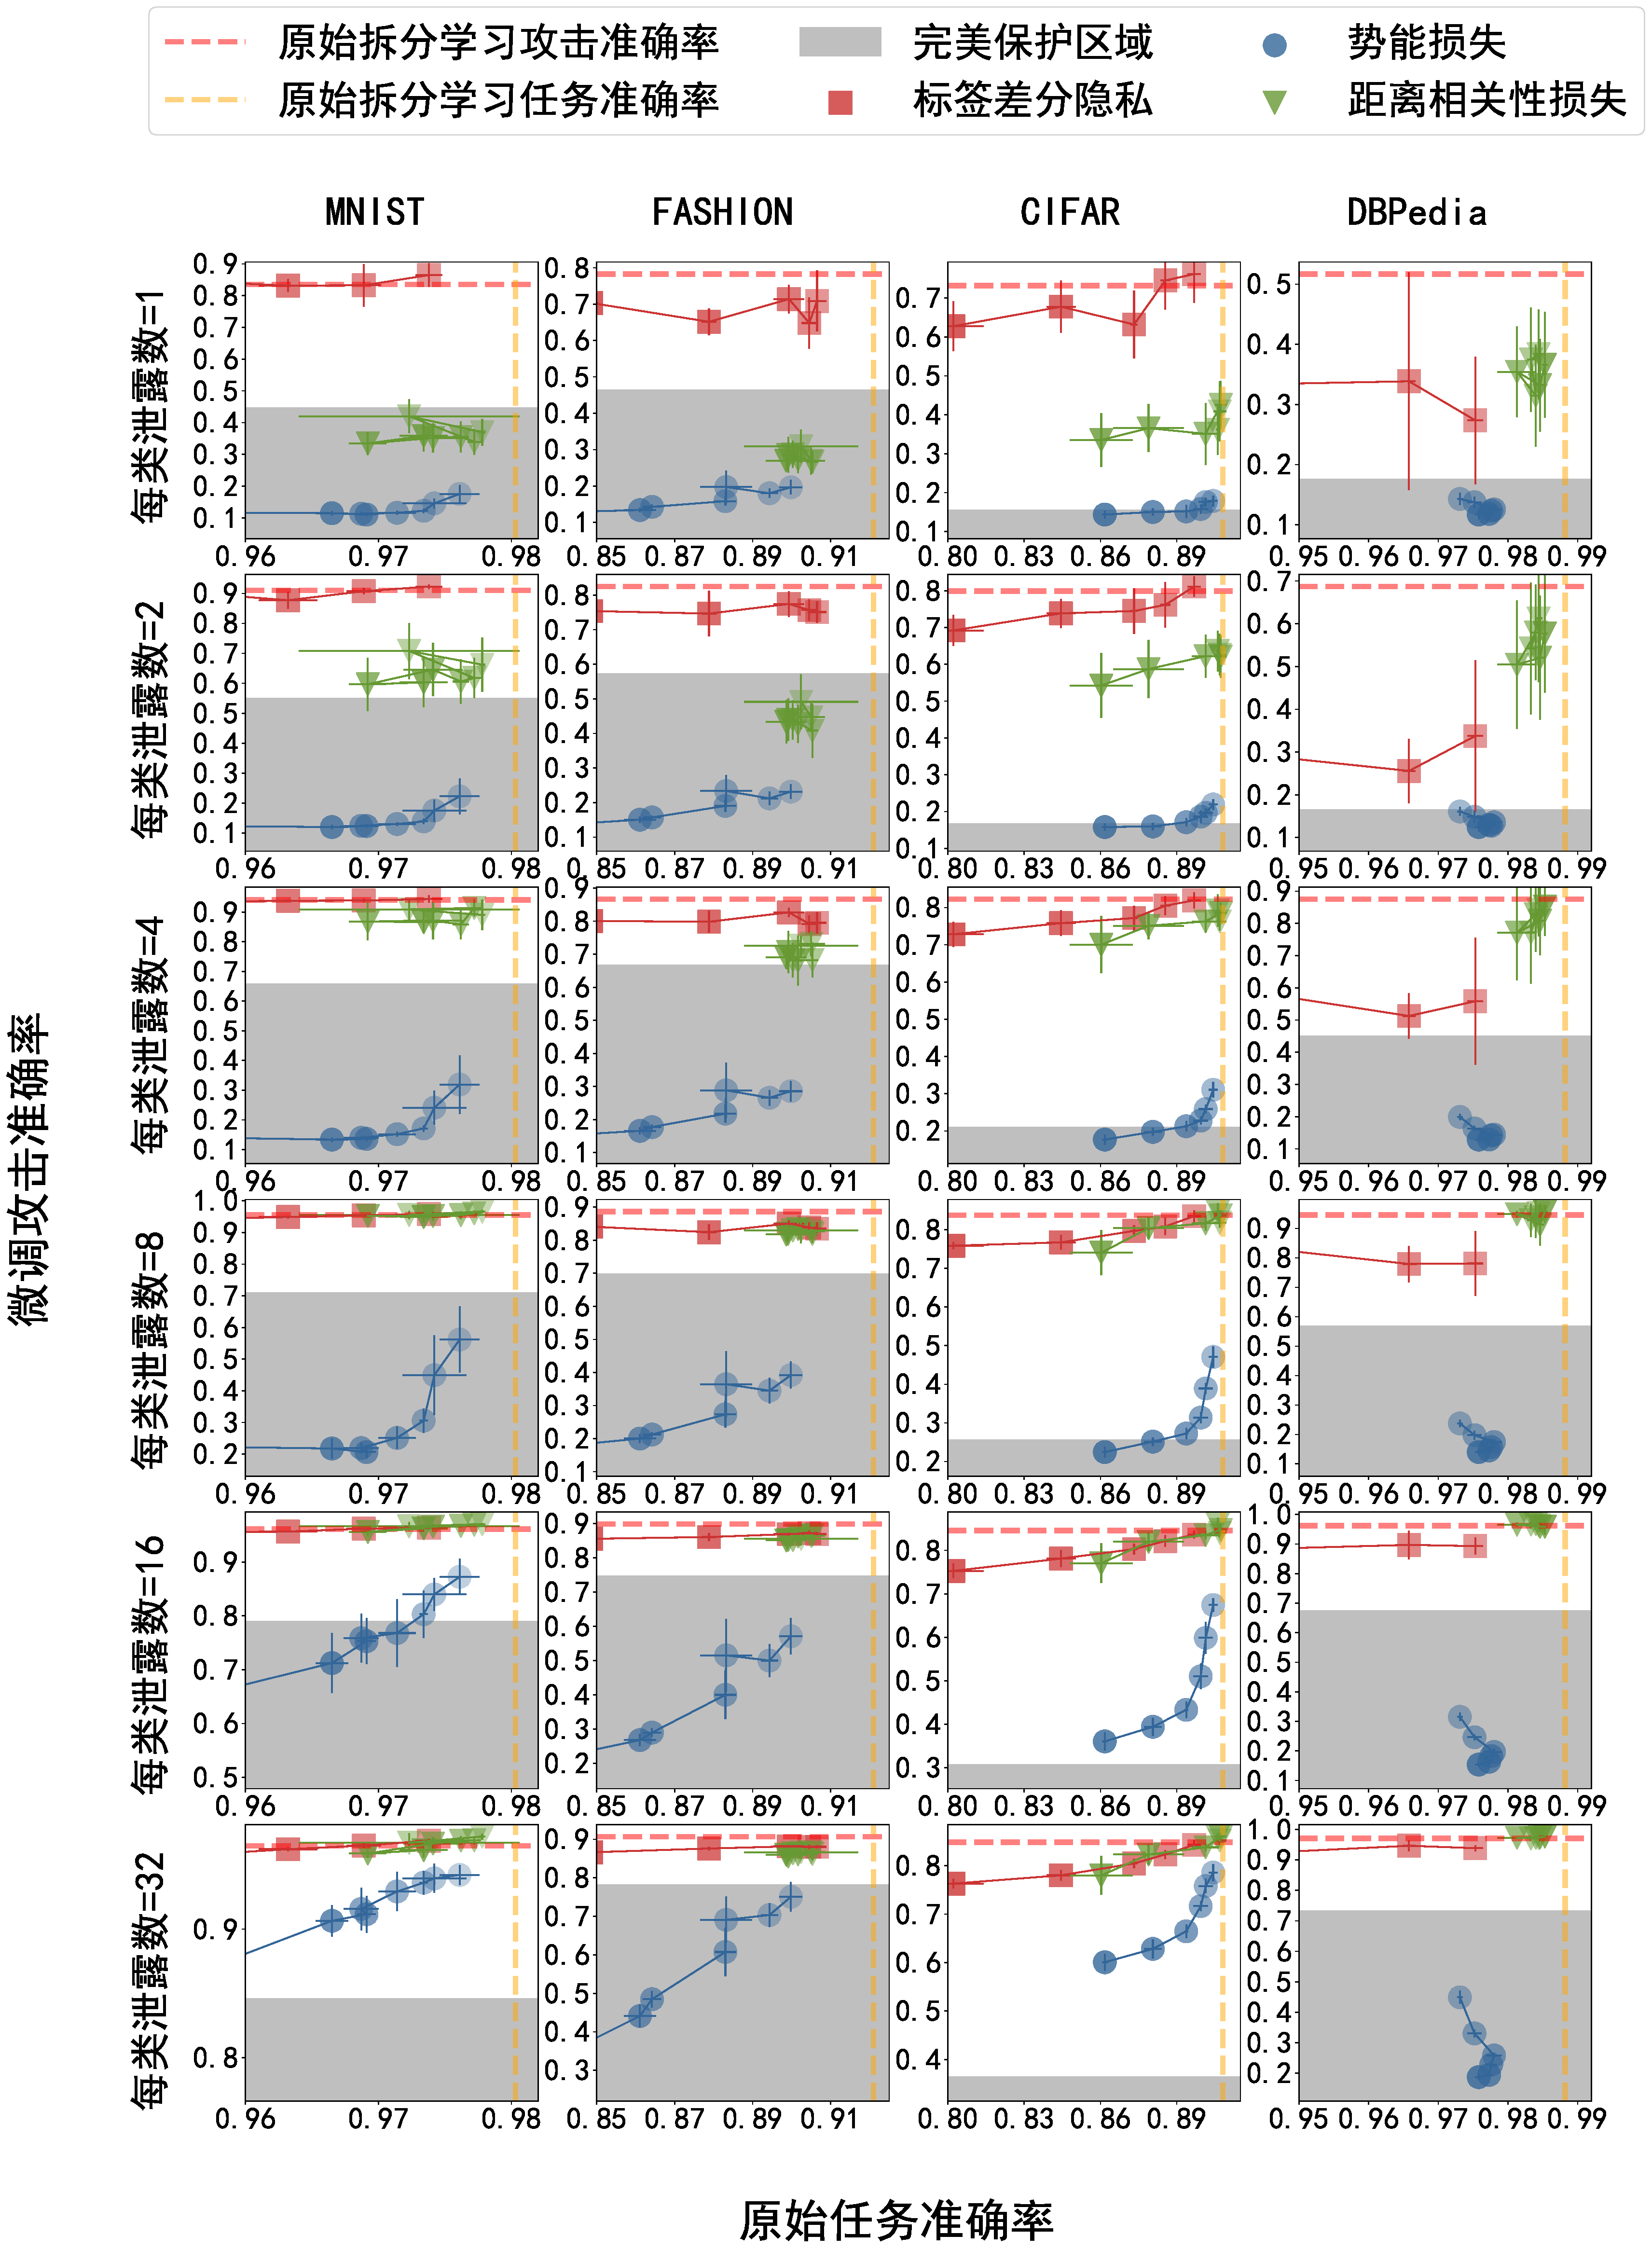
\includegraphics[width=1\linewidth]{Z_Resources/peloss_fine-tuning}
    \caption{拆分层为最后一层时原始任务准确率与微调攻击准确率对比图}
    \label{fig:peloss:fine-tuning}
\end{figure}


\begin{figure}[h!]
    \centering
    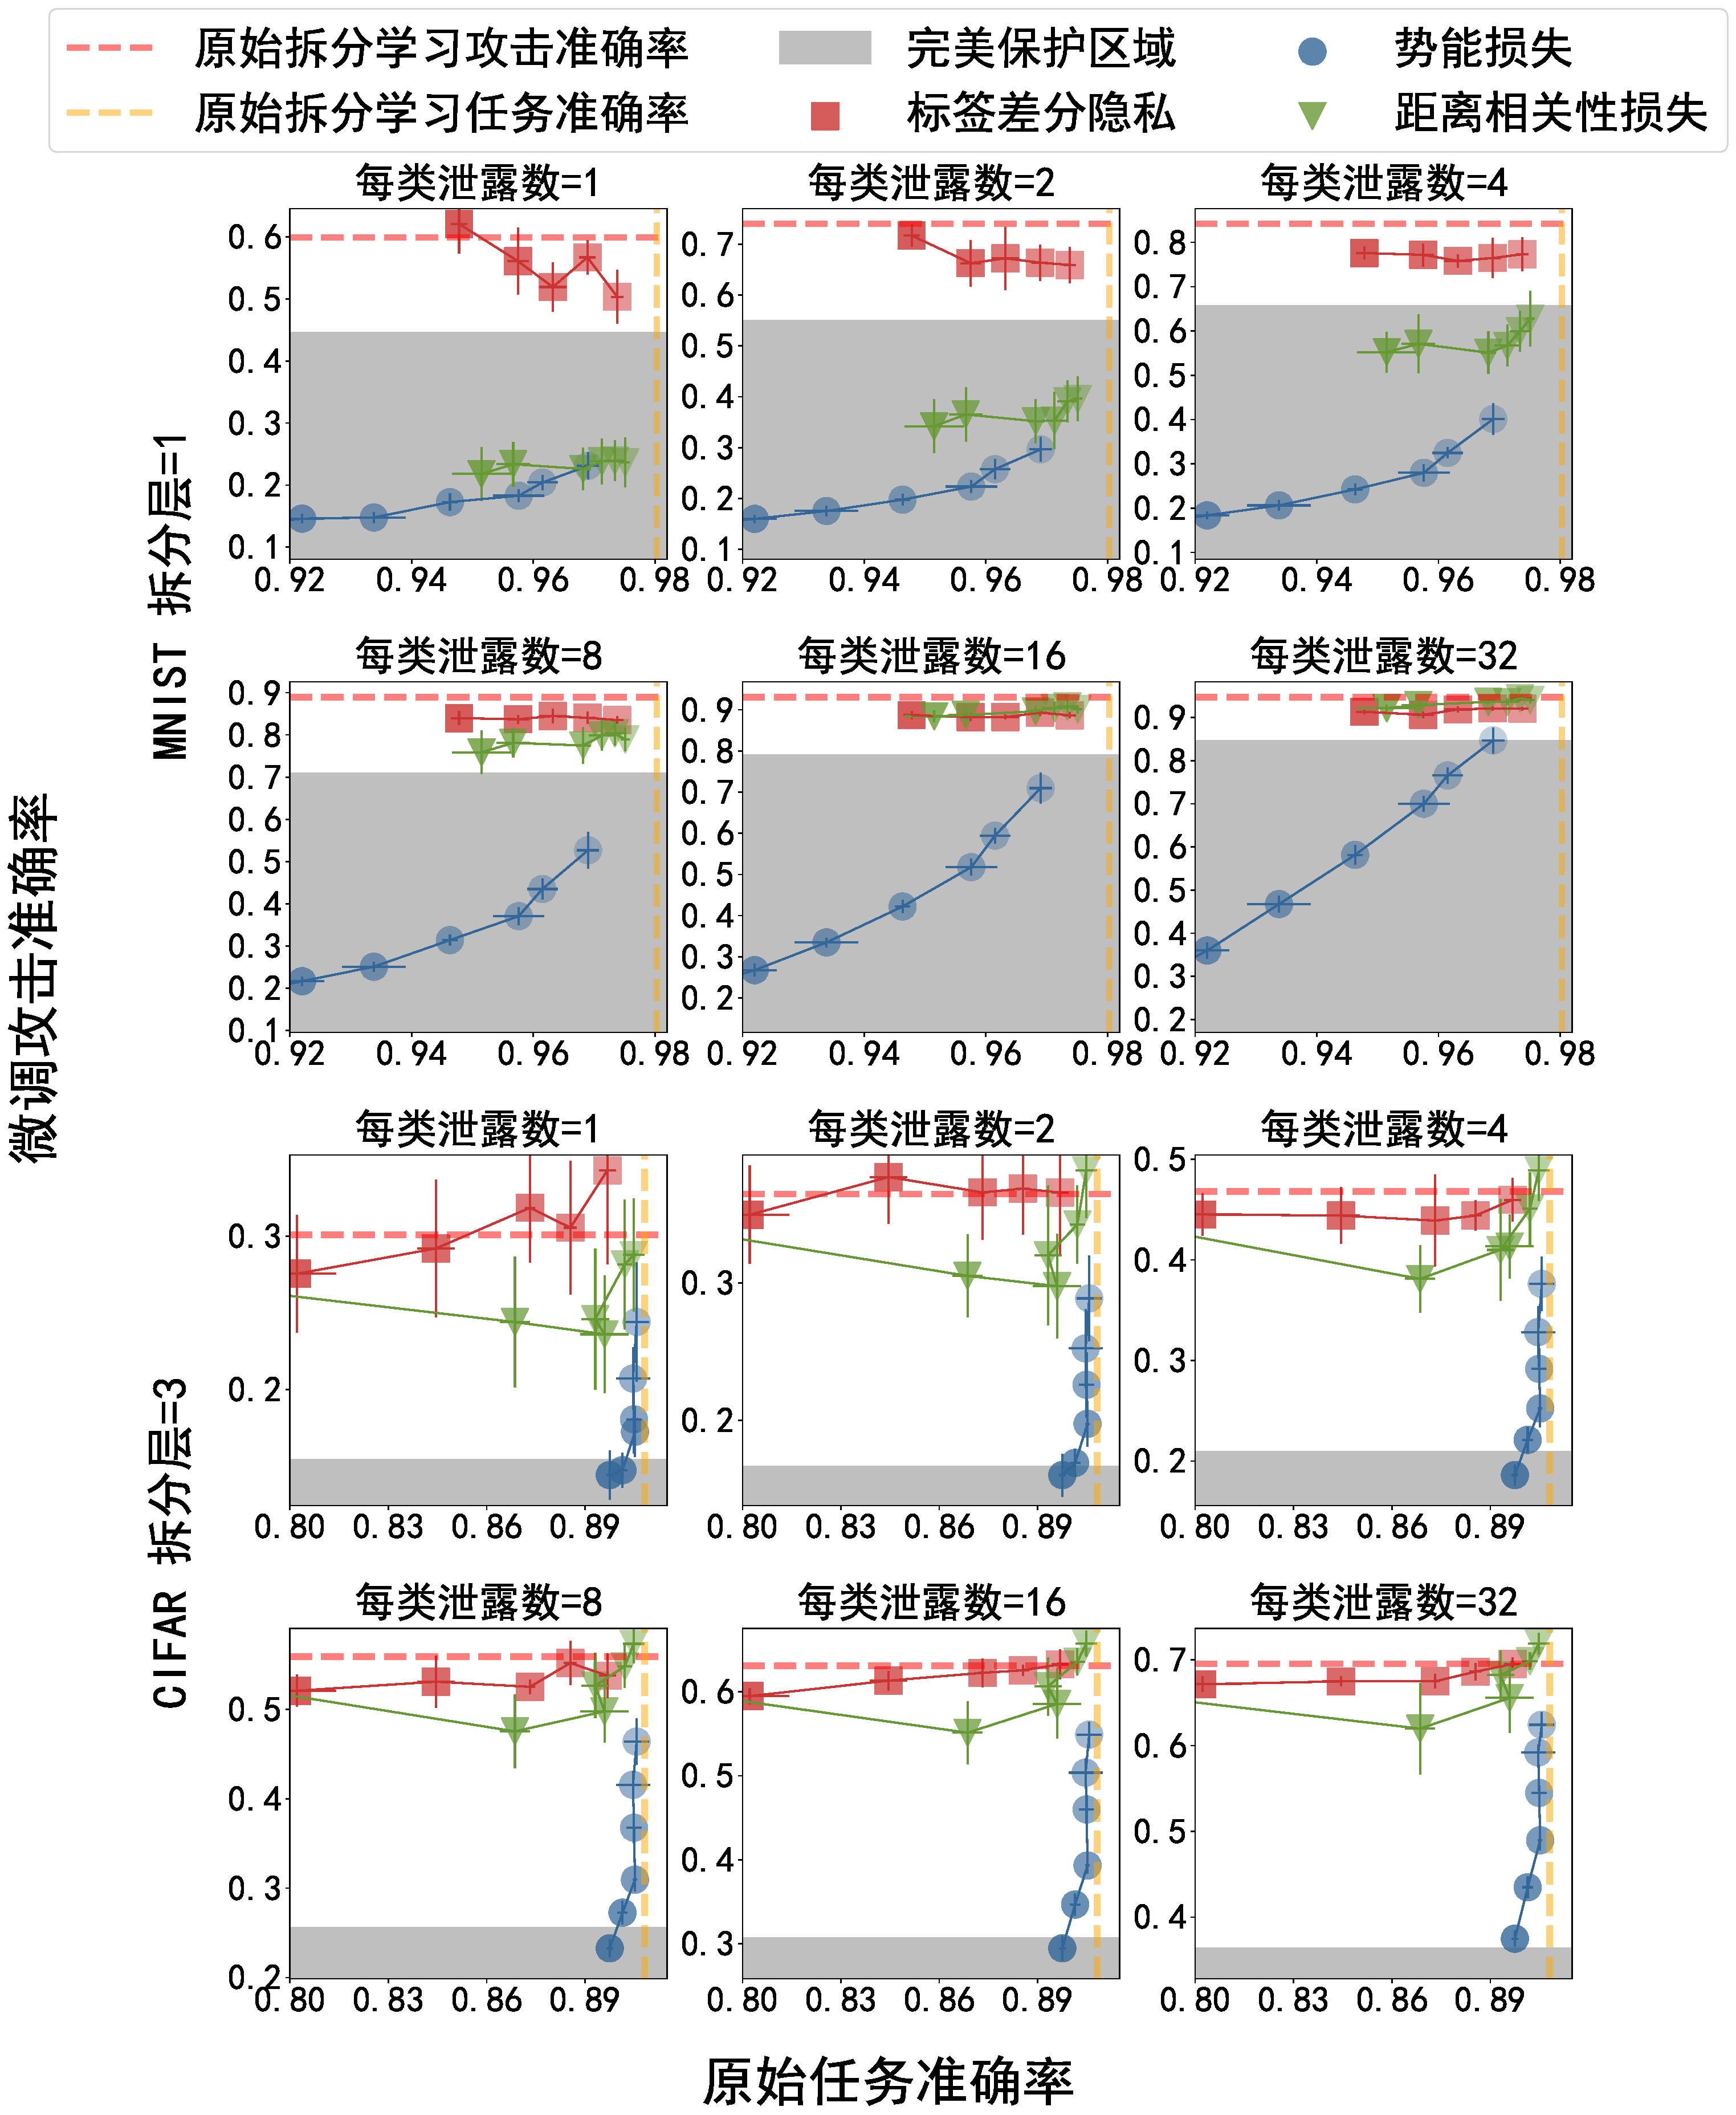
\includegraphics[width=0.85\linewidth]{Z_Resources/peloss_fine-tuning-middle}
    \caption{拆分层为中间层时原始任务准确率与微调攻击准确率对比图}
    \label{fig:peloss:fine-tuning-middle}
\end{figure}


\subsection{聚类攻击}
\begin{figure}[h!]
    \centering
    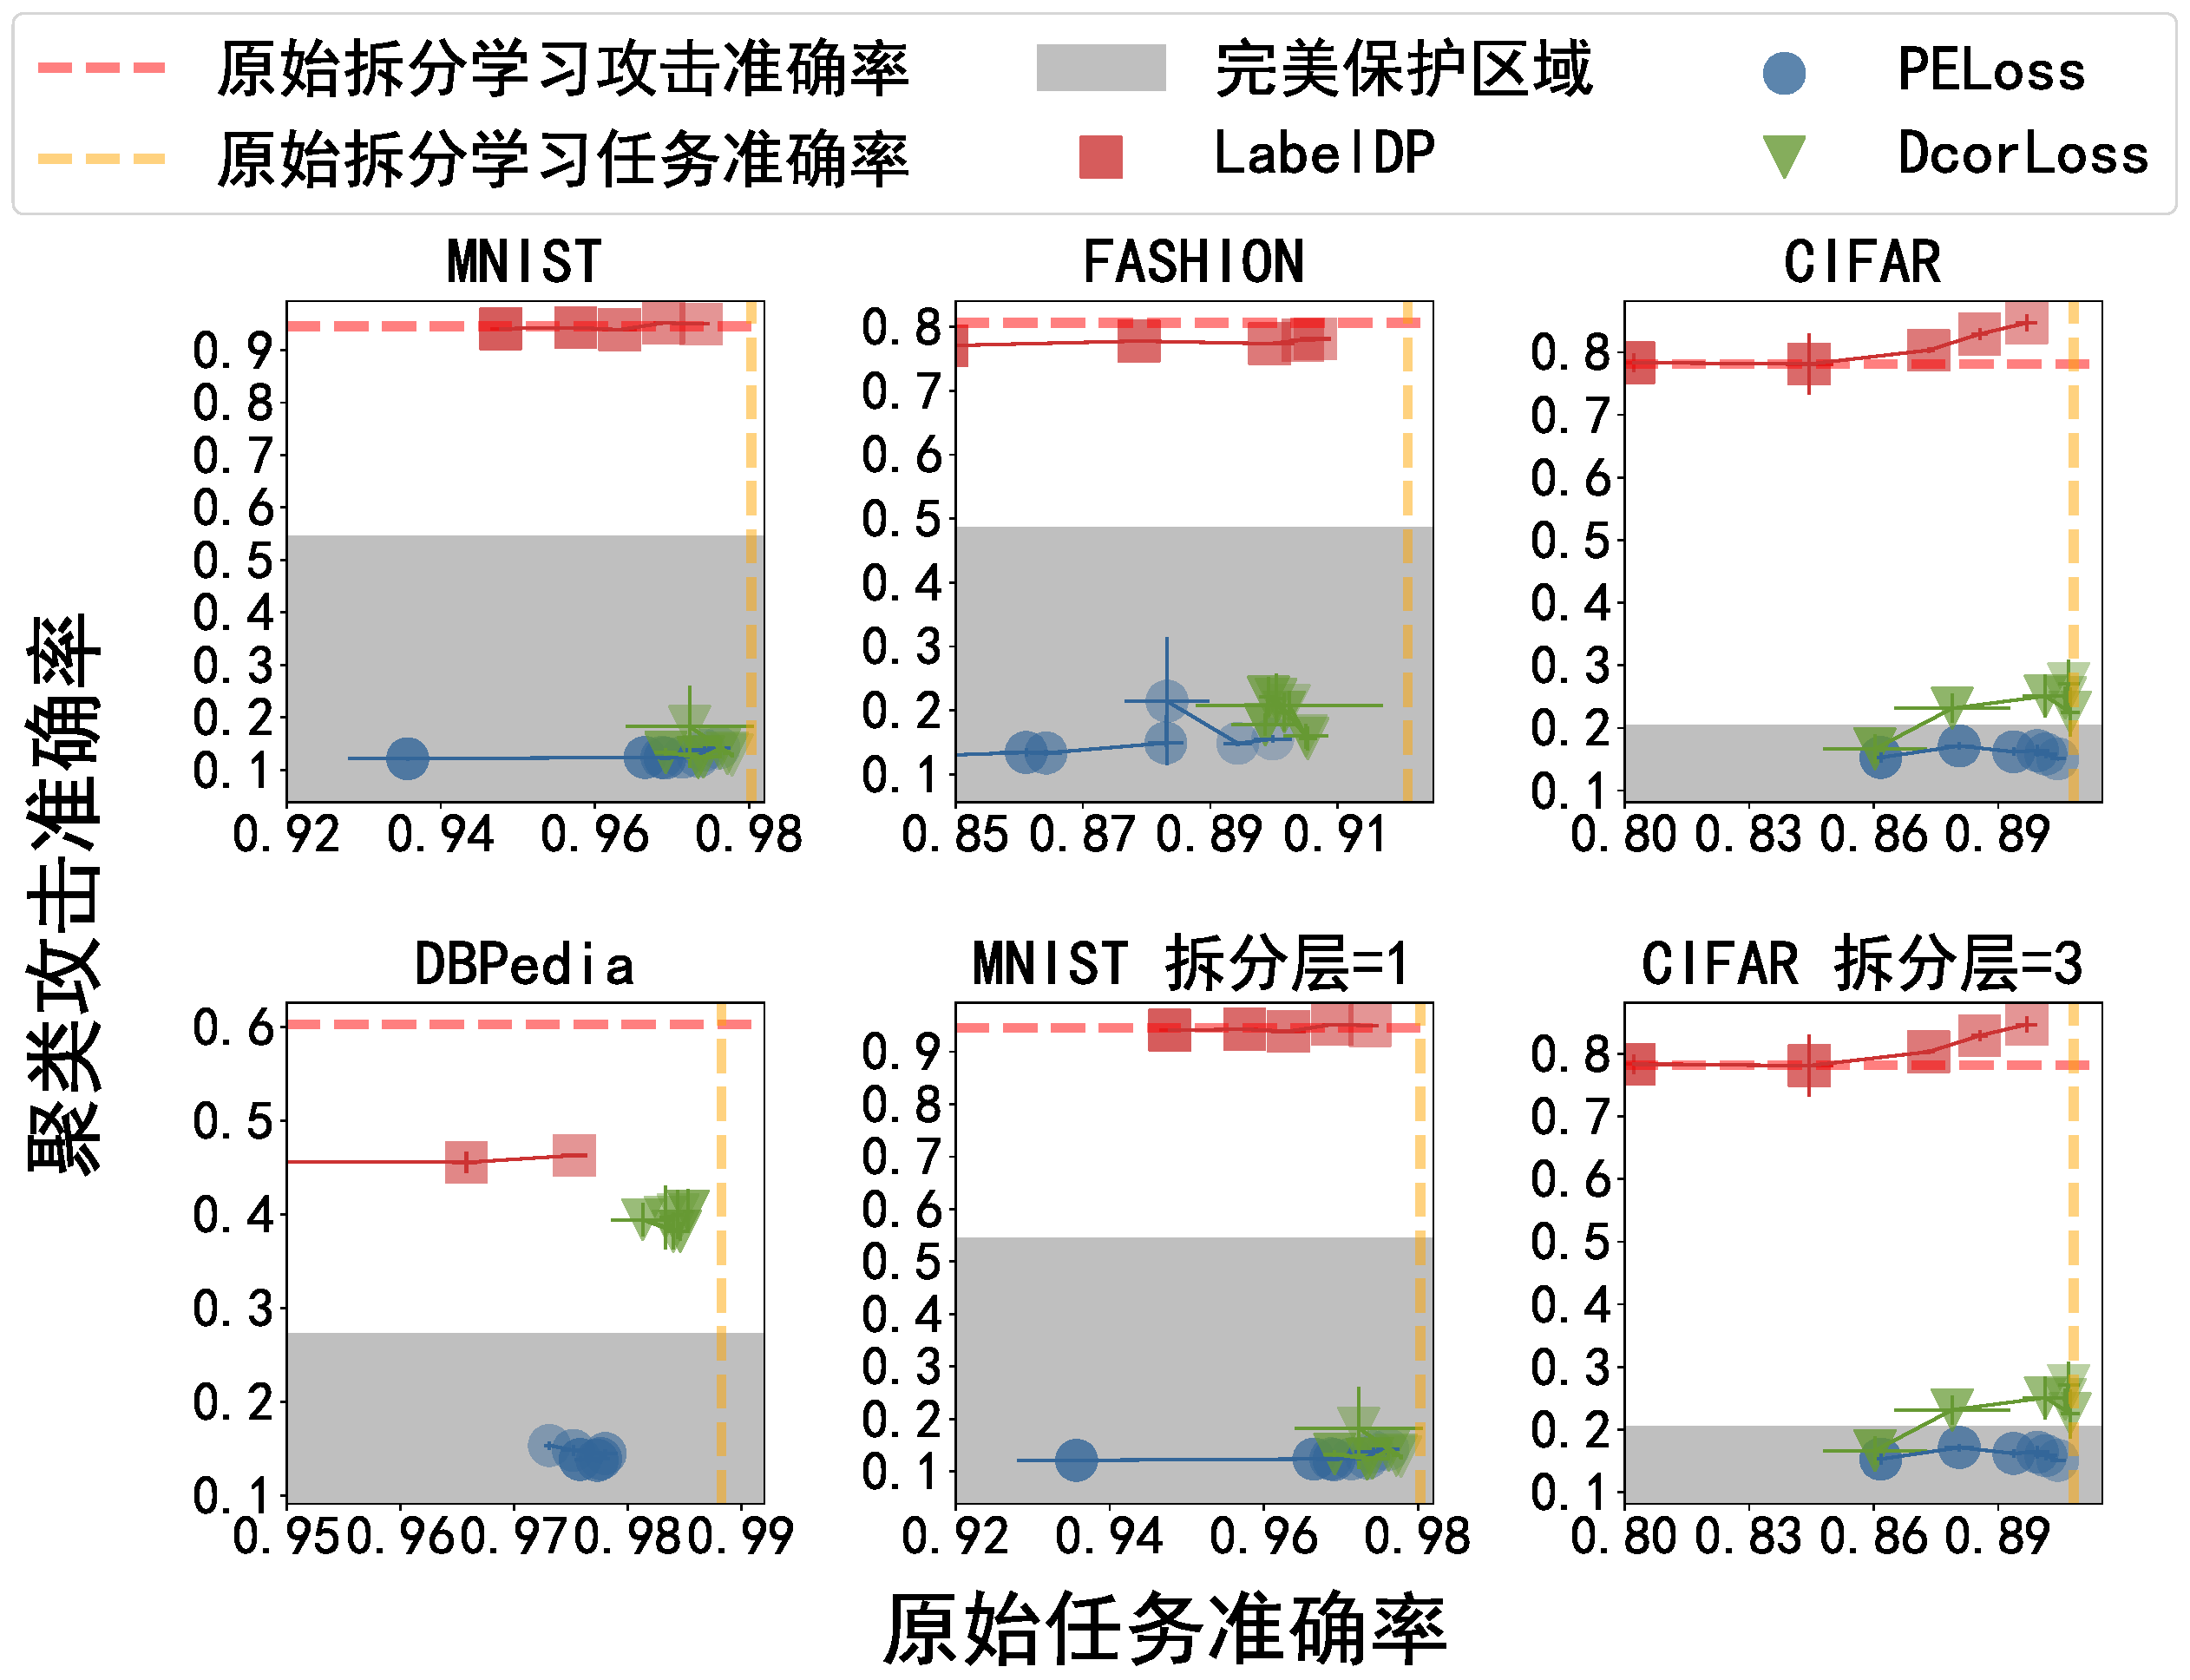
\includegraphics[width=0.8\linewidth]{Z_Resources/peloss_cluster-attack-both}
    \caption{原始任务准确率与聚类攻击准确率对比图}
    \label{fig:peloss:clustering}
\end{figure}

我们测量了模型在测试集上的准确率,以及攻击者无标签数据(整个测试集,均超过1万个样本)上进行聚类攻击得到的模型的准确率。
全部结果汇报在\autoref{fig:peloss:clustering}中。
%
由于聚类结果本身并不与实际的标签类别相对应,我们通过匈牙利匹配算法(Hungarian Matching Algorithm)~\cite{kuhn_1955_hungarian}找到准确率最高的类别映射关系并汇报该准确率。
该准确率计算公式可以表示为:
\begin{equation}
    \max\limits_{k_1,\cdots,k_C \in \text{Permutation}(1,\cdots,C)} \dfrac{\sum_{i=1}^C c_{i,k_i}}{\sum_{i,j=1}^C c_{i,j}},
\end{equation}
其中 $C$表示样本总数,$c_{i,j}$ 表示第 $i$ 个簇中实际标签是 $j$ 的样本数量, $1 < i, j \le C$。

%
实验结果表明,势能损失在所有的情况下均实现了完美保护,大幅领先于其他对比方法。
也就是说攻击者直接在泄漏的无标签数据上聚类得到的效果高于在拆分层表征上聚类得到的效果。
%
而标签差分隐私在对抗聚类攻击上效果不佳,相比于原始的拆分学习,未呈现出明显的保护作用。


\subsection{在拆分层之前攻击}
\begin{figure}[h!]
    \centering
    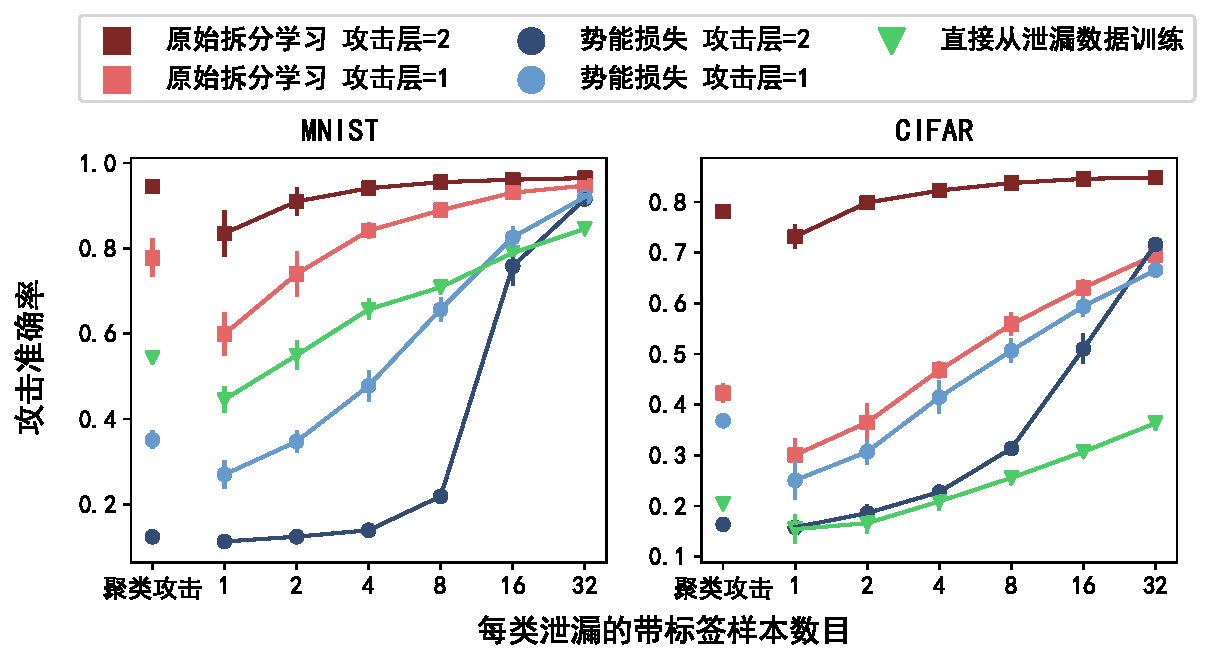
\includegraphics[width=0.85\linewidth]{Z_Resources/peloss_attack-layer}
    \caption{攻击层在拆分层之前时原始任务准确率与模型补全攻击准确率对比图}
    \label{fig:peloss:attack-layer}
\end{figure}

在之前的模型补全攻击实验中,我们假设攻击者使用了拆分层的表征进行攻击。
如果攻击者可以获取并操纵整个底部模型,则他也可以在拆分层之前的层进行攻击,也就是获取拆分层之前的隐层表征来微调模型或聚类。
%
因此,我们在MNIST和CIFAR任务中考察了攻击者在拆分层之前的层攻击的情况。
我们将拆分层设置为模型最后一个隐层,然后将MNIST任务的攻击层设置在第一个隐层处,将CIFAR-10任务的攻击层设置在第二个残差块(Residual Block)之后。
%
对于该实验,势能损失的系数被选取为$\alpha=4$。
%
我们在\autoref{fig:peloss:attack-layer}呈现在拆分层之前攻击的实验结果。

可以看到,在拆分层之前攻击可以让攻击效果有所提升,但是依然比无保护的拆分学习的攻击效果要低很多。
%
这是由于势能损失在训练过程中作用于拆分层的表征上而非之前的表征,因此拆分层之前的层的表征分布可能与标签关联性更大,使得攻击者更容易对其进行训练。

\subsection{拆分层维度的影响}
\begin{figure}[h!]
    \centering
    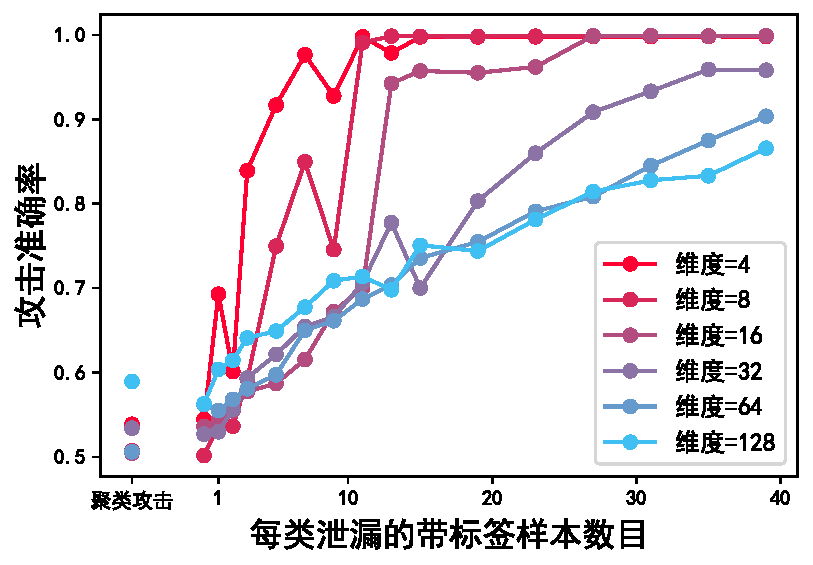
\includegraphics[width=0.7\linewidth]{Z_Resources/peloss_mnist-subclass2}
    \caption{拆分层维度对模型补全攻击准确率的影响}
    \label{fig:peloss:bottom_dim}
\end{figure}

为了研究拆分层的维度对于攻击效果的影响,我们对MNIST数据集的01子集上(只保留0和1类别的样本)进行了实验,其结果被汇报在\autoref{fig:peloss:bottom_dim}中。
此时我们设置势能损失的系数$\alpha=1$。

从图中可以看出,较高的拆分层维度大体上让微调攻击变得更难了,特别在每类样本泄露数较多的情况下。
%
例如,拆分层仅仅为4维的时候,只需要每个类别10个样本就可以让攻击准确率达到100;
而拆分层维度为128时,每类泄露40个样本后攻击准确率也不到90\%。
这是因为对更高维度的数据(也就是隐层表征)进行分类时,自然需要更多的样本。
%
作为对比,在聚类攻击时,更高的拆分层维度并未降低攻击的效果,甚至反倒有所提高。
这可能与聚类攻击时样本数量庞大有关。



\subsection{拆分层表征分布分析}
%
为了分析拆分层表征的分布,我们在MNIST数据集上计算了同类别表征之间和不同类别表征之间的角距离的分布,并且呈现在\autoref{fig:peloss:angular-distance} 中。
%
对于势能损失和距离相关性损失,我们分别把系数设置为$\alpha=1$和$\alpha=0.5$,这两者的原始任务效果基本相同。
%
图中可以看出,无论是否是同类别,抑或是属于训练集或者测试集,势能损失方法的样本表征间的角距离都接近$\pi/2$。
也就是说,无论两个表征是异类的或是同类的表征,它们都几乎相互正交。
%
对于距离相关性损失, 角距离则呈现出一个双峰分布,峰值靠近$0$和$\pi$。
并且同类别的样本表征对的角距离在靠近0的分布明显增加,导致保护效果变差。
%
而原始拆分学习中,同类别的表征之间的角距离则明显小于不同类别的表征之间的角距离,因此攻击准确率较高。


\begin{figure}[h!]
    \centering
    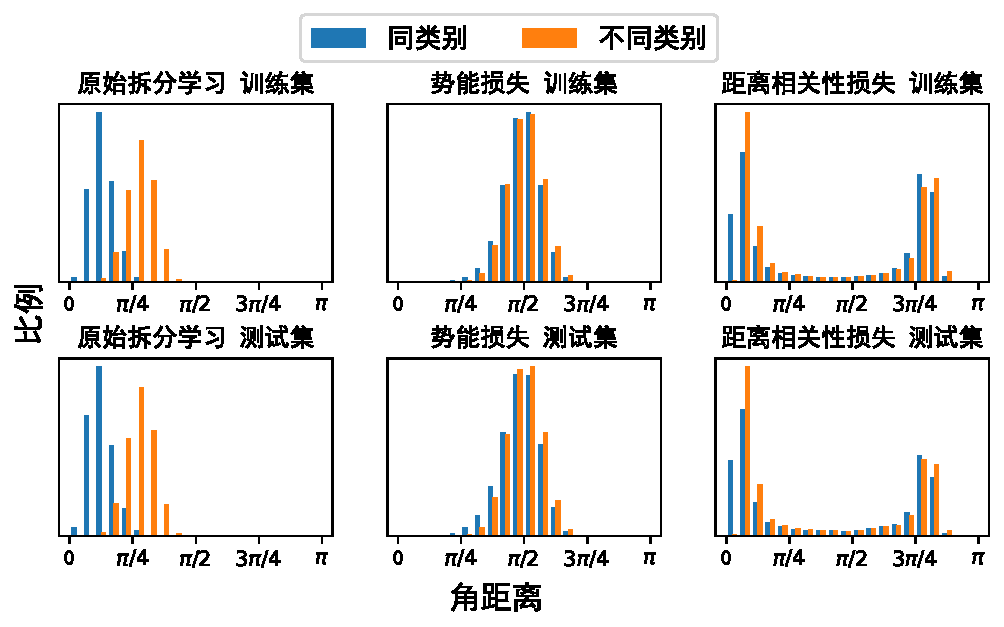
\includegraphics[width=0.8\linewidth]{Z_Resources/peloss_angular-distance}
    \caption{同类别和不同类别的隐层表征之间的角距离分布}
    \label{fig:peloss:angular-distance}
\end{figure}

为了更直观地呈现拆分层表征的分布,我们使用了t-SNE降维~\cite{van_2008_tsne}对拆分层表征进行可视化,呈现在\autoref{fig:peloss:tsne}中。
%
可以看到,原始拆分学习的拆分层表征呈现出明显的聚类性质,各个类别之间的表征可以很容易地被划分开。
%
而加入了势能损失后,不同类别的表征的分布的t-SNE投影融为一体,难以区分。
%
而距离相关性损失则呈现出了较为奇怪的分布,其分布被分为多个小块,而每个小块内都对应某个类别,且单个类别可能对应多个块。
由于同类表征间仍有一定程度的集聚效应,因此其安全性低于势能损失。

\begin{figure}[h!]
    \centering
    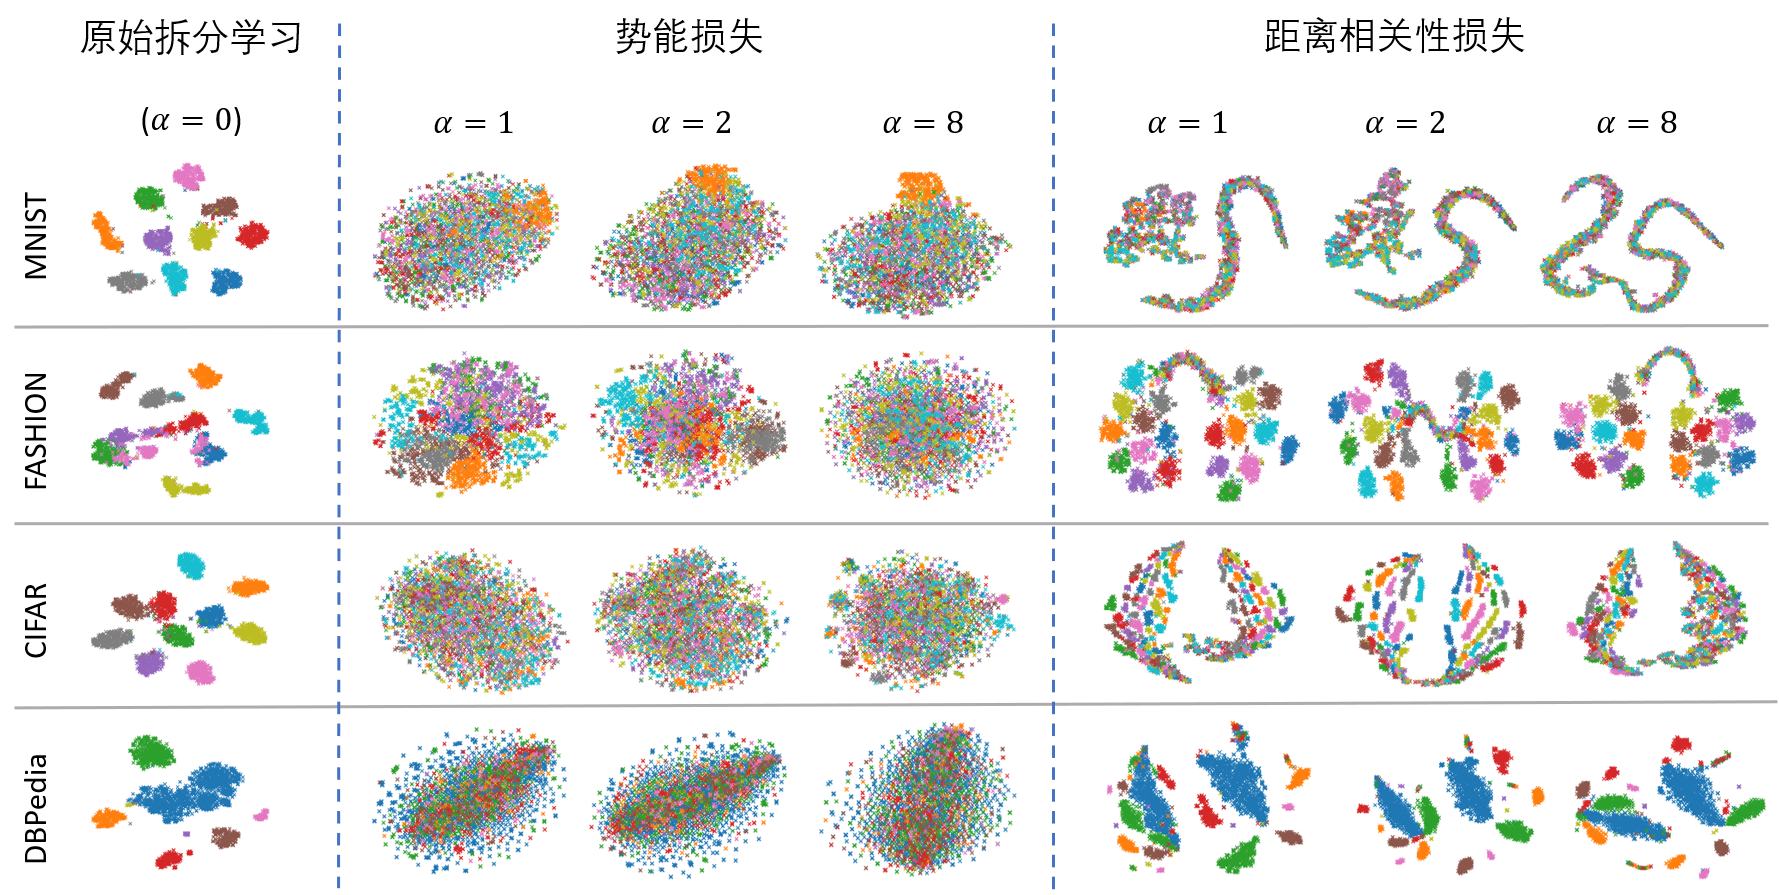
\includegraphics[width=1\linewidth]{Z_Resources/peloss_tsne}
    \caption{势能损失和距离相关性损失的隐层分布t-SNE降维}
    \label{fig:peloss:tsne}
\end{figure}


\subsection{在Transformer架构模型上的补充实验}
\begin{figure}[h!]
    \centering
    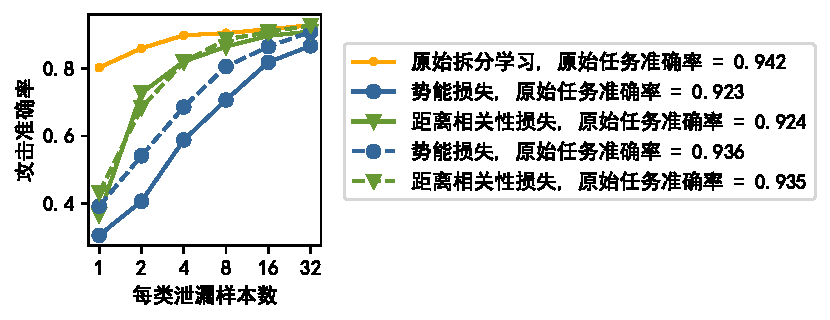
\includegraphics[width=1\linewidth]{Z_Resources/peloss_vegetable-primary}
    \caption{Vegetable Images数据集下不同泄露样本数和攻击准确率的对比}
    \label{fig:peloss:vegetable}
\end{figure}
为了进一步验证势能损失在Transformer结构的模型上的效果,我们在蔬菜图像~\cite{vegetable_2021}数据集上使用视觉Transformer(ViT, Vision Transformer)模型~\cite{alexey_2021_vit}进行了部分实验。
%
蔬菜图像数据集包含21000张图片,分为15个类别,其图片大小为$128\times 128 \times 3$。
%
我们将ViT模型的分块大小(Patch Size)设置为$16\times 16$,隐层大小为256,层数为4,注意力头(Attention Heads)个数为8。
%
实验结果呈现在\autoref{fig:peloss:vegetable}中,可以看出,势能损失在ViT模型上依然显著领先于对比的距离相关性损失。